%%%%%%%%%%%%%%%%%%%%%%%%%%%%%%%%%%%%%%%%%%%%%%%%%%%%%%%%%%%%%%%%%%%%%%%%%%%%%%%%%%%%%%%%%%%%%%%%%%%%%%%%%%%%%%%%%%%%%%%%%%%%%%%%%%%%%%%%%%%%%%%%%%%%%%%%%%%
% This is just an example/guide for you to refer to when submitting manuscripts to Frontiers, it is not mandatory to use frontiers.cls nor frontiers.tex  %
% This will only generate the Manuscript, the final article will be typeset by Frontier after acceptance.                                                 %
%%%%%%%%%%%%%%%%%%%%%%%%%%%%%%%%%%%%%%%%%%%%%%%%%%%%%%%%%%%%%%%%%%%%%%%%%%%%%%%%%%%%%%%%%%%%%%%%%%%%%%%%%%%%%%%%%%%%%%%%%%%%%%%%%%%%%%%%%%%%%%%%%%%%%%%%%%%

%%% Version 2.0 Generated 2013/09/12 %%%
%%% You will need to have the following packages installed: datetime, fmtcount, etoolbox, fcprefix, which are normally inlcuded in WinEdt. %%%
%%% In http://www.ctan.org/ you can find the packages and how to install them, if necessary. %%%

%\documentclass{frontiersENG} % for Engineering articles
\documentclass{frontiersSCNS} % for Science articles
%\documentclass{frontiersMED} % for Medicine articles

\usepackage{url,lineno}
\usepackage{graphicx}
\linenumbers

% Leave a blank line between paragraphs in stead of using \\

\copyrightyear{2013}
\pubyear{2013}

\def\journal{Neuroinformatics}%%% write here for which journal %%%
\def\DOI{}
\def\articleType{Methods}
\def\keyFont{\fontsize{8}{11}\helveticabold }
\def\firstAuthorLast{Nunez-Iglesias {et~al.}} %use et al only if is more than 1 author
\def\Authors{Juan Nunez-Iglesias\,$^{1,2,*}$, Ryan Kennedy\,$^{1,3}$, Stephen M. Plaza\,$^{1}$, Anirban Chakraborty\,$^{4}$ and William T. Katz\,$^1$}
% Affiliations should be keyed to the author's name with superscript numbers and be listed as follows: Laboratory, Institute, Department, Organization, City, State abbreviation (USA, Canada, Australia), and Country (without detailed address information such as city zip codes or street names).
% If one of the authors has a change of address, list the new address below the correspondence details using a superscript symbol and use the same symbol to indicate the author in the author list.
\def\Address{$^{1}$FlyEM project, HHMI Janelia Farm Research Campus, Ashburn, VA, USA \\
$^{2}$ Present address: Life Sciences Computation Centre, Victorian Life Sciences Computation Initiative, Carlton, VIC, Australia \\
$^{3}$ Department of Computer and Information Science, School of Engineering and Applied Sciences, University of Pennsylvania, Philadelphia, PA, USA \\
$^{4}$ Video Computing Group, Department of Electrical Engineering, University of California at Riverside, Riverside, CA, USA}
% The Corresponding Author should be marked with an asterisk
% Provide the exact contact address (this time including street name and city zip code) and email of the corresponding author
\def\corrAuthor{Juan Nunez-Iglesias}
\def\corrAddress{Life Sciences Computation Centre, Victorian Life Sciences Computation Initiative, Carlton, VIC, Australia}
\def\corrEmail{juan.n@unimelb.edu.au}

% \color{FrontiersColor} Is the color used in the Journal name, in the title, and the names of the sections.


\begin{document}
\onecolumn
\firstpage{1}

\title[learned agglomeration]{Graph-based Active Learning of Agglomeration (GALA): a Python library to segment 2D and 3D neuroimages.}
\author[\firstAuthorLast]{\Authors}
\address{}
\correspondance{}
\extraAuth{}% If there are more than 1 corresponding author, comment this line and uncomment the next one.
%\extraAuth{corresponding Author2 \\ Laboratory X2, Institute X2, Department X2, Organization X2, Street X2, City X2 , State XX2 (only USA, Canada and Australia), Zip Code2, X2 Country X2, email2@uni2.edu}
\topic{Python in Neuroscience II}% If your article is part of a Research Topic, please indicate here which.

\maketitle

%%%%%%%%%%%%%%%%%%%%%%%%%%%%%%%%%%%%%%%%%%%%%%%%%%%%%%%%%%%%%%%%%%%%%%%%%%%%%%%%%%%%%%%%%%%%%%%%%%%%%%%%%%%%%%%%%%%%%%%%%%%%%%%%%%%%%%%%%%%%%%%%%%%%%%%%%%%%%%%%%%%%%%%%%%%%%%%%%%%%%%%%%%%%%%%%%%%%%%%%%%%%%%%%%%%%%%%%%%%%%%%%%%%%%%%
%%% The sections below are for reference only.
%%%
%%% For Original Research Articles, Clinical Trial Articles, and Technology Reports the following sections are mandatory:
%%% Abstract, Introduction, Material and Methods, Results, and Discussion.
%%% Please note that the Material and Methods section can be placed in any of the following ways: before Results, before Discussion or after Discussion.
%%%
%%% For Clinical Case Studies the following sections are mandatory: Abstract, Introduction, Background, Discussion, and Concluding Remarks.
%%%
%%% For all other article types there are no mandatory sections.
%%%%%%%%%%%%%%%%%%%%%%%%%%%%%%%%%%%%%%%%%%%%%%%%%%%%%%%%%%%%%%%%%%%%%%%%%%%%%%%%%%%%%%%%%%%%%%%%%%%%%%%%%%%%%%%%%%%%%%%%%%%%%%%%%%%%%%%%%%%%%%%%%%%%%%%%%%%%%%%%%%%%%%%%%%%%%%%%%%%%%%%%%%%%%%%%%%%%%%%%%%%%%%%%%%%%%%%%%%%%%%%%%%%%%%%

\begin{abstract}

The aim in high-resolution connectomics is to reconstruct complete neuronal connectivity in a tissue.
Currently, the only technology capable of resolving the smallest neuronal processes is electron microscopy (EM).
Thus, a common approach is to perform automatic segmentation of EM images, followed by manual proofreading by experts to fix errors.
We developed an algorithm and software library to not only improve the accuracy of the initial automatic segmentation, but also point out the image coordinates where it is likely to have made errors.
Our software, called gala (graph-based active learning of agglomeration), improves the state of the art in agglomerative image segmentation.
It is implemented in Python and makes extensive use of the scientific Python stack (numpy, scipy, networkx, scikit-learn, scikit-image, and others).
We present here the software architecture of the gala library, and discuss several designs that we consider would be generally useful for other segmentation packages.
We also discuss the limitations of the gala library and how we intend to address them.

%%% Leave the Abstract empty if your article falls under any of the following categories: Editorial Book Review, Commentary, Field Grand Challenge, Opinion or specialty Grand Challenge.
\section{}
%As a primary goal, the abstract should render the general significance and conceptual advance of the work clearly accessible to a broad readership. References should not be cited in the abstract.


\tiny
 \keyFont{ \section{Keywords:} connectomics, python, electron microscopy, image segmentation, machine learning} %All article types: you may provide up to 8 keywords; at least 5 are mandatory.
\end{abstract}


\section{Introduction}

% For Original Research Articles, Clinical Trial Articles, and Technology Reports the introduction should be succinct, with no subheadings.
%
%For Clinical Case Studies the Introduction should include symptoms at presentation, physical exams and lab results.
%

Connectomics, the elucidation of complete neuronal circuits, requires resolutions as low as 5-10nm to distinguish the smallest neuronal processes, but also fields of view of hundreds of micrometers or larger, as neurons can easily span those distances.
This size disparity results in large image volumes of at least 10 gigavoxels and often orders of magnitude larger than even this.
Neurons can then be thought of as segments in this image.
Finally, by marking the position of pre- and post-synaptic sites in the image, one can obtain the shapes, locations, and connectivity of all the neurons in an enormous image volume.

Until recently, the rate-limiting step has been the proofreading of the automatic segmentation \cite{Chklovskii:2010df}

We recently developed a new machine learning-based algorithm for image segmentation \citep{NunezIglesias:2013cd}.
Description of GALA algorithm.
GALA is state of the art. outperformed previous agglomeration methods in EM and natural image segmentation. top-ranked in SNEMI3D challenge, above 2D-specific methods.

We briefly present the Python application programming interface (API) and the command-line interface (CLI), before delving more deeply into particularly useful design choices, and finally discussing the current limitations of the library and future directions.


\section{API}


\subsection{Python API}

Main gala pipeline

Ability to implement related algorithms: mean, median, flat learning, LASH

Highlight evaluate module

Mention NeuroProof


\subsection{Command-line interface}

Use SNEMI3D example.


\section{Design}


\subsection{N-dimensional array support}
Many segmentation libraries assume 2D or 3D data (REFS).
Thanks to numpy's ndarray support, and because all operations in our algorithm depend only on the definition of the local neighborhood, it was feasible to design gala to be dimension-agnostic.
By defining a neighbor function, that takes in a pixel index, a shape, and a connectivity parameter, and calling this function instead of manually computing on indices, gala segments numpy array volumes of arbitrary dimension.

(Usage examples of neighbors function and nd support.)


\subsection{Feature managers and feature caches}

An example of a critical feature when determining the probability that two segments should be merged is the average pixel-level probability of boundary (REFS).
As segments are merged, the shared surface between them and their common neighbors increases, thereby making the average a more reliable estimate of the true probability of a boundary.
Recomputing the mean from scratch, however, results in quadratic time complexity, because we are repeatedly iterating over the same pixels after each merge.
Therefore, a more efficient strategy is to cache a sum of the pixel probabilities and the count of pixels examined.
Then, when two boundaries are combines, their probability sums are added together, as are their counts, and the new average probability can be computed by dividing the new sum by the new count, in constant time.
This caching has turned a quadratic operation into a linear one.

The above concept can be generalized to *any* feature.
We found that, in many cases, caching intermediate computations dramatically improved the time complexity of feature computation.
For example, to compute the *variance* of the pixel probabilities, we must cache the sum of the *squared* pixel probabilities, along with simple sum and counts.
To compute a histogram, we cache the unnormalised histogram, and each bin is summed when two boundaries are combined.

We therefore devised a single class, which we call a feature manager, that is responsible for defining the cached values, and for computing the feature vector from the cached values.


\subsection{Classifier abstraction}

Given the vast heterogeneity of our initial feature space, we wished to use a random forest (RF) as our classifier of choice.
When we started building gala, \texttt{scikit-learn}, the present gold-standard in machine learning Python libraries, did not include RF.
We therefore decided to use Vigra, a C++ image analysis and machine learning library with Python bindings.
However, we recognized that a cross-compatible interface across libraries would allow rapid testing of various machine learning techniques.
We therefore built a wrapper around Vigra to match \texttt{scikit-learn}'s estimator interface, particularly the \texttt{fit()}, \texttt{predict()}, and \texttt{predict\_proba()} methods.

Because of this, it is trivially easy to use different classifiers for the learning and agglomeration steps of \texttt{gala}.
In particular, we have been able to use the recently vastly improved \texttt{RandomForestClassifier} from \texttt{scikit-learn} version 0.14 with zero code changes.

In short, by using established interfaces, we were able to future-proof our software.
We recommend that anyone looking to build software in the Python ecosystem take a long look at related libraries to match interfaces as close as possible.


\section{Discussion}


\subsection{Alternate backends}

Gala supports an alternative backend, NeuroProof, that uses a C++ RAG based on the Boost Graph Library with Python bindings (Plaza and Parag, in preparation).

\subsection{Complete gold standard requirement}

As currently implemented, gala requires a fully segmented volume from which to learn.
In our experiments, this has become the major bottleneck to getting segmentation of new data started.
Therefore, a major priority in gala development going forward is the ability to "mask" volumes so that partial ground truth can be used.

\subsection{Memory and time inefficiency}

Numerous improvements and low-hanging fruit are possible.

Firstly, we currently store feature caches and compute feature vectors as separate arrays.
This results in a huge time overhead for large graphs due to memory allocation, and also in memory usage because of the dictionaries required to store all the separate arrays.
However, because we are performing a hierarchical agglomeration, we know that the number of nodes and edges is bounded by twice the initial number.
Therefore, we can pre-allocate an initial array of shape \texttt{(2 * n\_nodes, cache\_size)} for the node feature caches, and similarly for the edges, and use an incremental indexing scheme to keep track of which node or edge in the hierarchy uses which row of the array.

Additionally, the graph currently stores indices to the voxels comprising each node and boundary, which is unnecessary.
Space and time can be saved by keeping only a single voxel and rebuilding nodes using a flood fill.

Finally, we chose the heavy \texttt{Graph} class of the NetworkX library for its flexibility and fast node addition and removal.
However, this is ultimately unnecessary: we can just keep the original supervoxel graph using a much more efficient structure (such as \texttt{scipy.sparse.csc\_graph}, and maintain a merge tree.
The graph at any level of the hierarchy can be rapidly constructed from this.


\section{Conclusions}


%%% Use this if adding the figures directly in the mansucript, if so, please remember to also upload the files when submitting your article
%%% There is no need for adding the file termination, as long as you indicate where the file is saved. In the examples below the files (logo1.jpg and logo2.eps) are in the Frontiers LaTeX folder
%%% If using *.tif files convert them to .jpg or .png

\begin{figure}
\begin{center}
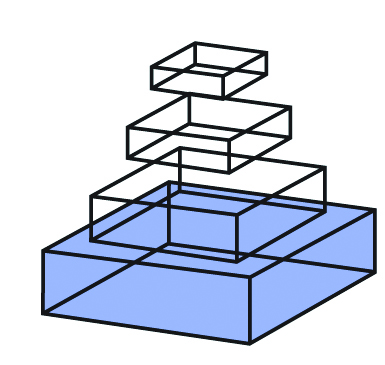
\includegraphics[width=3.5cm]{logo1}% This is a *.jpg file
\end{center}
 \textbf{\refstepcounter{figure}\label{fig:01} Figure \arabic{figure}.}{ Enter the caption for your figure here.  Repeat as  necessary for each of your figures }
\end{figure}

\begin{figure}
\begin{center}

\includegraphics[width=3.5cm]{logo2}% This is an *.eps file
\end{center}
 \textbf{\refstepcounter{figure}\label{fig:02} Figure \arabic{figure}.}{ Enter the caption for your figure here.  Repeat as  necessary for each of your figures }
\end{figure}

% \textbf{Figure 1.}{ Enter the caption for your figure here.  Repeat as  necessary for each of your figures.}\label{fig:01}% If you don't add the figures in the LaTeX files, please upload them when submitting the article.
%
%%% Frontiers will add the figures at the end of the provisional pdf automatically %%%



\bibliographystyle{frontiersSCNS} % for Science and Engineering articles
%\bibliographystyle{frontiersinMED} % for Medicine articles
\bibliography{frontiers.bib}

\end{document}
